%----------------------------------------------------------------------------------------
%	SECTION 1
%----------------------------------------------------------------------------------------

\section{The Closure Operator of a Matroid.}

\begin{definition}
    Let $M$ be a matroid on a set $E$, we define a mapping $\cl:2^E \rightarrow
    2^E$ called the \textbf{closure operator} of $M$ by the rule:
    \begin{equation*}
        \cl(X)=\{e \in E : \rank{(X \cup e)}=\rank{X}\}
    \end{equation*}
    For all $X \in E$. We call  $\cl{X}$ the \textbf{closure}, or the
    \textbf{span} of $X$ in  $M$.
\end{definition}

\begin{example}\label{1.14}
    \item[(1)] For any vector space $V$, and a vector  $v \in V$,  $v$ is in the
        span of a set of vectors  $\{v_1, \dots, v_n\}$ if the subspaces spanned
        by $\{v_1, \dots, v_n\}$ and $\{v_1, \dots, v_n,v\}$ have the same
        dimension. Indeed, the span of a subset of vectors ion $V$ is the closure
        operator for the matroid  $M[V]$.

    \item[(2)] In example \ref{1.12}(2), we have $\cl{\emptyset}=Z$,
        $\cl{\{1,3,5\}}=\{1,2,3,4,5\}$, and $\cl{\{4,5,6\}}=X$.
\end{example}

\begin{lemma}\label{1.4.1}
    Let $M$ be a matroid on a set  $E$, then for every $X \subseteq E$,
    $\rank{X}=\rank{(\cl{X})}$.
\end{lemma}
\begin{proof}
    Let $B$ be a basis of  $X$, then for each  $x \in \com{(\cl{X})}{X}$,
    $\rank{(B \cup x)}=\rank{X}=\rank{B} \leq \rank{(B \cup x)}$. Then
    $\rajnk{(B \cup x)}<|B \cup x|$, so that $B \cup x$ is a dependent set. This
    makes  $B$ a basis of  $\cl{X}$.
\end{proof}

\begin{lemma}\label{1.4.2}
    The closure operator of a matroid $M$ on a set  $E$ satisfies the following
    for all  $X,Y \subseteq E$:
    \begin{enumerate}
        \item[(CL1)] $X \subseteq \cl{X}$.

        \item[(CL2)] If $X \subseteq Y$, then  $\cl{X} \subseteq \cl{Y}$.

        \item[(CL3)] $\cl{X}=\cl{(\cl{X})}$.

        \item[(CL4)] If $x \in E$, and  $y \in \com{\cl{(X \cup x)}}{\cl{X}}$,
            then $x \in \cl{X \cup y}$.
    \end{enumerate}
\end{lemma}
\begin{proof}
    By definition of closure, we have that $\rank{X \cup x}=\rank{X}$ for all $x
    \in X$, so  $x \in \cl{X}$. Now suppose that $X \subseteq Y$, and let  $x
    \in \com{(\cl{X})}{X}$, then $\rank{(X \cup x)}=\rank{X}$. Now if $B$ is a
    basis of  $X$, then it is a basis for  $X \cup x$. Then  $Y \cup x$ has a
    basis  $B'$ which contains $\com{B}{x}$. Then it follows that $\rank{Yc \cup
    x}=\rank{Y}$, so that $x \in \cl{Y}$. So $\cl{X} \subseteq \cl{Y}$.

    Notice also that $\cl{X} \subseteq \cl{(\cl{X})}$. Then for $x \in
    \cl{(\cl{X})}$, $\rank{(\cl{X} \cup x)}=\rank{(\cl{X})}=\rank{X}$, by lemma
    \ref{1.4.1}, now we have that $\rank{X} \leq \rank{)X \cup x} \lewq
    \rank{(\cl{X} \cup x)}$, so equality holds and $x \in \cl{X}$.

    Now suppose that $y \in \com{{(\cl{(X \cup x)})}}{\cl{X}}$, then $\rank{X
    \cup x \cup y}=\rank{X \cup x}$, and $\rank{X \cup y} \neq \rank{X}$. Then
    by the corollary to lemma \ref{1.3.1}, we het $\rank{(X \cup
    y)}=\ranl{X}+1$. Thus we have that $\rank{X}+1=\rank{(X \cup y)} \leq
    \rank{(X \cup x \cup y)}=\rank{(X \cup y)}=\rank{X}+1$, so by equality, we
    get $\rank{(X \cup x \cup y)}=\rank{X \cup y}$, so that $x \in \cl{(X \cup
    y)}$.
\end{proof}

\begin{lemma}\label{1.4.3}
    Let $M$ be a matroid on a set $E$. Let $X \subseteq E$, and  $x \in E$. If
    $X$ is an independent set, and $X \cup x$ a dependent set, then $x \in
    \cl{X}$.
\end{lemma}
\begin{proof}
    We have that $X \cup x \notin \Ic$, is dependent, so that for  $y \in X \cup
    x$,  $y \in \cl{\com{(X \cup x)}{y}}$. Now, if $y=x$, we are done as
    $\com{(X \cup x)}{y}=X$. On the otherhand, if $y \neq x$, then  $\com{(X
    \cup x)}{y}=(\com{X}{y}) \cup x$, so $y \in \com{\cl{((\com{X}{y}) \cup
    x)}}{\cl{(\com{X}{y})}}$. Therefore, $x \in \cl{((\com{X}{y}) \cup
    y)}=\cl{X}$.
\end{proof}

\begin{theorem}\label{1.4.4}
    Let $E$ be a set and  $\cl:2^E \rightarrow 2^E$ be a mapping satisfying
    (CL1)-(CL4). If $\Ic=\{X \subseteq X : x \notin \cl{(\com{X}{x})}, \text{
    for all } x \in X\}$, then $\Ic$ is the collection of independent sets of a
    matroid  $M$ on  $E$ having  $\cl$ as its closure operator.
\end{theorem}
\begin{proof}
    We have $\emptyset \in \Ic$. Now, let $I \in \Ic$ with  $I' \subseteq  I$,
    then for any  $x \in I$, we have  $x \notin \cl{(\com{I}{x})}$, and
    $\cl{(\com{I'}{x})} \subseteq \cl{(\com{I}{x})}$, so $x \notin
    \cl{(\com{I}{x})}$. Therefore $I' \in \Ic$.

    Now let  $I,I' \in \Ic$ with  $|I|<|I'|$, and suppose there is no  $e \in
    \com{I'}{I}$ such that $I \cup e \in \Ic$, and suppose additionally that for
    all pairs of  $I$ and  $I'$, that  $|I \cap I'|$ is maximal. Choose then a
    $y \in \com{I'}{I}$ and take $\com{I'}{y}$. Suppose that $I \subseteq
    \cl{(\com{I'}{y})}$, then $\cl{I} \subseteq \cl{(\com{I'}{y})}$, so that $y
    \notin \cl{\(\com{I}{y})}$, therefore by the above lemma we have that $I
    \cup y \in \Ic$, which contradicts our assumption. So we get that  $\cl{I}
    \notsubseteq \cl{(\com{I'}{y})}$, and there is some $t \in I$, and  $t
    \notin \cl{(\com{I'}{y})}$. Now, $t \in \com{I}{I'}$, and $(\com{I'}{y})
    \cup t \in \Ic$. Now $|I \cap(\com{I'}{y}) \cup t|>|I \cap I'|$, so that $x
    \in \com{((\com{I'}{y}) \cup t)}{I}$, making $I \cup x \in \Ic$, but  $x \in
    \com{I'}{I}$, a contradiction. Therefore such an $e$ stated in the
    assumption must exist. This makes  $M$ into a matroid with  $\Ic$ as its
    collection of independent sets.

    Now suppose that $x \in \com{(\cl{X})}{X}$ and that $B$ is a basis of  $X$.
    Then  $\rank{(X \cup x)}=\rank{X}$, and $B \in \Ic$, and  $B \cup x \notin
    \Ic$. Then it follows that  $x \in \cl{B}$ by the above lemma. Likewise, if
    $x \in \com{{(\cl{X})}}{X}$ and $B$ is a basis of  $X$, then  $B \cup y
    \notin \Ic$ for all  $y \in \com{X}{B}$. So again we get that $X \subseteq
    \cl{B}$, so $\cl{X} \subseteq \cl{B}$. Thus $x \in \cl{B}$ so that $B \cup x
    \in \Ic$, making  $B \cup x$ a basis of  $X \cup x$, and $\rank{(X \cup
    x)}=|B|=\rank{X}$. Therefore $\cl$ is the closure operator of $M$.
\end{proof}
\begin{corollary}
    For any set $E$, the mapping $\cl:2^E \rightarrow 2^E$ is the closure
    operator for a matroid on $E$ if, and only if it satisfies (CL1)-(CL4).
\end{corollary}

\begin{definition}
    We define a matroid $M$ on a set  $E$ to be the pair  $(E,\cl)$ where
    $\cl:2^E \rightarrow 2^E$ is a mapping satisfying the following:
    \begin{enumerate}
        \item[(CL1)] $X \subseteq \cl{X}$.

        \item[(CL2)] If $X \subseteq Y$, then  $\cl{X} \subseteq \cl{Y}$.

        \item[(CL3)] $\cl{X}=\cl{(\cl{X})}$.

        \item[(CL4)] If $x \in E$, and  $y \in \com{\cl{(X \cup x)}}{\cl{X}}$,
            then $x \in \cl{X \cup y}$.
    \end{enumerate}
    We call $\cl$ the \textbf{closure operator} of  $M$, and we call  $\cl{X}$
    th \textbf{closure}, or \textbf{span} of $X$ in  $M$.
\end{definition}

We have thge immediate lemma concerning the closure operator.

\begin{lemma}\label{1.4.5}
    Let $M$ be a matroid on a set $E$, then the following are true for all $X,Y
    \subseteq E$.
    \begin{enumerate}
        \item[(1)] If $X \subseteq \cl{Y}$, and $\cl{Y} \subseteq \cl{X}$, then
            $\cl{X}=\cl{Y}$.

        \item[(2)] If $Y \subseteq \cl{X}$, then $\cl{(X \cup Y)}=\cl{X}$.

        \item[(3)] The intersection of all flats containing $X$ is precisely
            $\cl{X}$.

        \item[(4)] $\rank{(X \cup Y)}=\rank{(X \cup \cl{Y})}=\rank{(\cl{X} \cup
            \cl{X})}=\rank{(\cl{(X \cup Y)})}$.

        \item[(5)] If $X \subseteq Y$,  and  $\rank{X}=\rank{Y}$, then
            $\cl{X}=\cl{Y}$.
    \end{enumerate}
\end{lemma}
\begin{proof}
    Let $X \subseteq Y$, and  $\cl{Y} \subseteq \cl{X}$, then we have $\cl{X}
    \subseteq \cl{(\cl{Y})}=\cl{Y}$, this shows equality.

    Now, if $Y \subseteq \cl{X}$, then for all $y \in Y$,  $\rank{(X \cup y)}=
    \rank{X}$, then by lemma \ref{1.3.2}, $\rank{(X \cup Y)}=\rank{X}$.

    To prove (3), let $\Fc=\bigcap_{X \subseteq F}{F}$ be the intersection of
    all flats $F$ containing  $X$. Then for each  $F$,  $\cl{F}=F$, by
    containment, this makes $\cl{X}=X$, so that $\cl{X} \subseteq \Fc$. On the
    otherhand, if $x \in \Fc$, then  $x \in F$, $F$, arbitrary. If $x \in \cl{X}$,
    then we are done, otherwise, $\rank{(X \cup x)}=\rank{X}+1$, but $\rank{(F
    \cup x)}=\rank{F}$, which makes $\rank{(X \cup x)}>\rank{X}$, which
    contradicts the rank properties. Therefore $x \in \cl{X}$. This makes $\Fc
    \subseteq \cl{X}$.

    Now, for (4), we have $Y \subseteq \cl{Y}$, so $\rank{(X \cup Y)} \leq
    \rank{(X \cup \cl{Y})} \leq \rank{(\cl{X} \cup \cl{Y})} \leq \rank{(\cl{(X
    \cup Y)})}=\rank{(X \cup Y)}$, since $e \in \cl{(X \cup Y)}$ implies
    $\rank{(X \cup Y \cup e)}=\rank{(X \cup Y)}$.

    Lastly, let $X \subseteq Y$ with  $\rank{X}=\rank{Y}$. First we have $\cl{X}
    \subseteq \cl{Y}$. Now if $y \in \cl{Y}$, then $\rank{(Y \cup
    y)}=\rank{Y}=\rank{X}$, then $\rank{(X \cup y)} \leq \rank{X}+1=\rank{Y}+1$.
    Now, if equality holds, then (R2) is contradicted, so we must have $\rank{(X
    \cup y)}<\rank{Y}+1$, so that $\rank{(X \cup y)}=\rank{Y}=\rank{X}$.
\end{proof}

We also have the additional definitions.

\begin{definition}
    if $M$ is a matroid on a set  $E$ with closure operator $\cl$, then we call
    a subset $X$ of  $E$ a  \textbf{flat} if $\cl{X}=X$. We call $X$ a
    \textbf{hyperplane} if it is a flat of rank $\rank{M}-1$, and we call $X$ a
     \textbf{spanning set} of $M$ if  $\cl{X}=E$. If $Y \subseteq \cl{X}$, we
     also say that $X$  \textbf{spans} $Y$.
\end{definition}

\begin{example}\label{1.15}
    \begin{figure}[h]
        \centering
        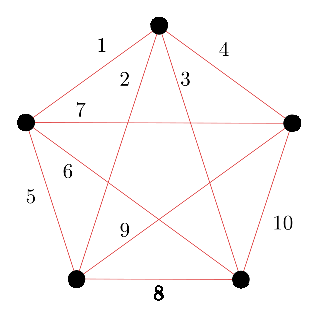
\includegraphics[scale=1.0]{Figures/Chapter1/closure_K_5.eps}
        \caption{}
        \label{fig_1.7}
    \end{figure}
    Consider the graphic matroid on $K_5$ labeled as in figure \ref{fig_1.7}.
    then $M(K_5)$ has $\emptyset$ as the unique flat of rank  $0$. The rank-$1$
    flats of $M(K_5)$ are the edges of $K_5$, the rank-$2$ flats of $M(K_5)$ are
    the edgesets of  $K_3$ along with pairs of adjacent edges of $K_5$. the
    rank-$3$ flats of $M(K_5)$ are teh hyperplanes of  $M(K_5)$, and consists of
    the edgesets of  $K_4$ along with edgesets that are isomorphic to the
    disjoint union $K_2 \cup K_3$. Finally, the rank-$4$ flat of $M(K_5)$ is
    $M(K_5)$ itself.
\end{example}

\begin{lemma}\label{1.4.6}
    let $M$ be a matroid on  $E$, and let  $X \subseteq E$. If  $x \in \cl{X}$,
    then $\cl{(X \cup x)}=\cl{X}$.
\end{lemma}

\begin{theorem}\label{1.4.7}
    Let $M$ be a matroid on  $E$, and let $X \subseteq E$. Then:
    \begin{enumerate}
        \item[(1)] $X$ is a spanning set if, and only if  $\rank{X}=\rank{M}$.

        \item[(2)] $X$ is a basis if, and only if  $X$ is a independent spanning
            set.

        \item[(3)] $X$ is a basis if, and only if it is a minimal spanning set.

        \item[(4)] $X$ is a hyperplane if, and only if it is a maximal
            nonspanning set.
    \end{enumerate}
\end{theorem}
\begin{proof}
    First, let $X$ be a spanning set of $M$, then $\cl{X}=E$, ten by lemma
    \ref{1.4.1}, $\rank{X}=\rank{(\cl{X})}=\rank{E}=\rank{M}$, so $X$ is a basis
    of  $M$. Conversely, if $\rank{X}=\rank{M}$, then for all $e \in E$,
    $\rank{(X \cup e)}=\rank{X}=\rank{M}$. This makes $\cl{X}=E$, and hence $X$
    is spanning.

    Now, if  $X$ is a basis, then  $\rank{X}=\rank{M}$, and $X$ is independent,
    so  $X$ is an independent spanning set. Conversely, if  $X$ is an
    independent spanning set, we have  $\rank{X}=\rank{M}$, and by theorem
    \ref{1.3.4}, $X$ must be a basis.

     let $X$ be a minimal spanning set. Then  $\rank{X}=\rank{M}$, and if $x \in
     X$, then  $\com{X}{x}$ is not spanning. so by theorem \ref{1.4.8}, $x
     \notin \cl{(\com{X}{x})}$, this makes $X$ independent, and hence  $X$ is a
     basis. Now, if  $X$ is a basis, then  $X$ is spanning and independent. Then
      $\cl{X}=E$. Now let $x \in X$, then  $\rank{(X \cup x)}=\rank{X}$, and
      $\rank{(\com{X}{x})} \leq \rank{X}$, if equality holds, then
      $\rank{(\com{X}{x})}=\rank{M}$, making $\cl{(\com{X}{x})}=E$, which
      contradicts the spanning of $X$. Therefore $\com{X}{x}$ cannot be
      spanning, making $X$ minimal.

      Lastly suppose that $X$ is a hyperplane, then it is a flat of rank
      $\rank{M}-1$; that is $\rank{X}=\rank{M}-1$, and $\cl{X}=X$. Now, if $x
      \in \com{E}{X}$, then $\rank{(X \cup x)}=\rank{X}+1=\rank{M}$, so that $X
      \cup x$ is not a flat, and hence not a hyperplane. Moreover, if $\rank{(X
      \cup x)}=\rank{M}$, then $E \subseteq \cl{X}$, making $X$ a spanning set.
      On the other hand, suppose that $X$ is a maximal nonspanning set. That is
      $\cl{(X \cup x)}=E$. Then $\rank{(X \cup x)}=\rank{M}$, hence $\rank{X}=
      \rank{M}-1$. Now, by maximality, we also have that $\cl{X} \neq E$, but
      that for any $x \in \cl{X}$, $\rank{(X \cup x)}=\rank{X}$, so that $x \in
      X$. Therefore  $\cl{X}=X$. This makes $X$ a flat of rank  $\rank{M}-1$,
      and hence a hyperplane.
\end{proof}

\begin{theorem}\label{1.4.8}
    Let $M$ be a matroid on a set  $E$. Then:
    \begin{enumerate}
        \item[(1)] $X$ is a circuit if, and only if  $X$ is a minimal nonempty
            set such that  $x \in \cl{(\com{X}{x})}$ for all $x \in X$.

        \item[(2)] $\cl{X}=X \cup \{x : x \in C \subseteq X \cup x,
            \text{ where } C \text{ is a circuit of } M\}$.
    \end{enumerate}
\end{theorem}
\begin{proof}
    The first statement mjust reasserts that circuits are minimal dependent
    sets. Now, for the second statement, suppose that $x \in \com{\cl{X}}{X}$,
    then $\rank{X \cup x}=\rank{X}$, so if $B$ is a basis of  $X$, then  $B \cup
    x$ is a dependent set. Therefore there exists a circuit  $C$ with  $x \in C
    \subseteq B \cup x$. Thus  $x \in C \subseteq X \cup x$. Conversly, if $C$
    is a circuit, ten by (1) and (CL2), $x \in \cl{(\com{C}{x})} \subseteq
    \cl{(\com{X}{x})}$.
\end{proof}

The above theorem motivates the following theorem.

\begin{theorem}[The Strong Circuit Elimination Axiom]\label{1.4.9}
    The collection $\Cc$ of circuits of a matroid satisfies the following:
    \begin{enumerate}
        \item[(C^\prime3)] If $C_1,C_2 \in \Cc$ with $e \in C_1 \cap C_2$, and $f
            \in \com{C_1}{C_2}$, then there exists a $C \in \Cc$ such that  $f
            \in C \subseteq \com{(C_1 \cup C_2)}{e}$.
    \end{enumerate}
\end{theorem}
\begin{proof}
    Notice that $e \in \cl{(\com{C_2}{e})}$ and that $\com{C_2}{e} \subseteq
    \com{(C_1 \cup C_2)}{\{e,f\}}$. Then $e \in \cl{(\com{(C_1 \cup
    C_2)}{\{e,f\}})}$, therfore we get $\cl{(\com{(C_1 \cup
C_2)}{\{e,f\}})}=\cl{(\com{(C_1 \cup C_2)}{f})}$. But $f \in \cl{(\com{C}{f})}
\subseteq \cl{(\com{(C_1 \cup C_2)}{f})}$, so $f \in
\cl{(\com{(C_1 \cup C_2)}{\{e,f\}})}$ Thus, by theorem \ref{1.4.8}, the matroid
of $\Cc$ has a circuit $C$ with $f \in C \subseteq \com{(C_1 \cup C_2)}{e}$.
\end{proof}
\begin{corollary}
    A collection $\Cc$ of subsets of a set  $E$ is the collection of circuits of
    a matroid if, and only if it satisfies the following:
    \begin{enumerate}
        \item[(C1)] $\emptyset \notin \Cc$.

        \item[(C2)] If $C_1, C_2 \in \Cc$, and $C_1 \subseteq C_2$, then
            $C_1=C_2$.

        \item[(C^\prime3)] If $C_1,C_2 \in \Cc$ with $e \in C_1 \cap C_2$, and $f
            \in \com{C_1}{C_2}$, then there exists a $C \in \Cc$ such that  $f
            \in C \subseteq \com{(C_1 \cup C_2)}{e}$.
\end{corollary}

\begin{lemma}\label{1.4.10}
    Let $M$ be a matroid on a set  $E$. Then the following are equivalent for
    any  $e \in E$.
    \begin{enumerate}
        \item[(1)] $e$ is in every basis of  $M$.

        \item[(2)] $e$ is in no circuit of  $M$.

        \item[(3)] If $X \subseteq E$ and  $e \in \cl{X}$, then $e \in X$.

        \item[(4)] $\rank{(\com{E}{e})}=\rank{E}-1$

        \item[(5)] $\com{E}{e}$ is a flat.

        \item[(6)] $\com{E}{e}$ is a hyperplane.

        \item[(7)] If $I$ is independent, then so is  $I \cup e$
    \end{enumerate}
\end{lemma}
\begin{proof}
    If $e$ is in any basis, of  $M$, then  $e$ cannot be in any dependent set,
    and hence no circuit.

    Now suppose that  $e$ is in no circuit, and that for  $X \subseteq E$, that
     $e \in \cl{X}$. Then if $e \notin X$,  $e \in \{x : x \in C \subseteq X
     \cup x \text{ where } C \text{ is a circuit of } M\}$. This makes $e$
     contained in a circuit contained in  $X \cup e$, which contradicts our
     supposition. So  $e \in X$.

     Now supposse that for  $X \subseteq E$, and  $e \in \cl{X}$, that $e \in
     X$. Then we get that  $\cl{X}=X$, so that $X$ is a flat of  $M$. Then
     $\rank{(X \cup e)}=\rank{X}$. Then notice that $E \subseteq E$, and that
     $e \in \cl{E}$, then we have $\rank{(\com{E}{e})}=\rank{E}-1$. This makes
     $\com{E}{e}$ a flat, since for any other $f \in \com{E}{e}$,
     $\rank{((\com{E}{e}) \cup f)}=\rank{(\com{E}{e})}=\rank{E}-1$. We also get
     that $\com{E}{e}$ is a hyperplane.

     Now, if $\com{E}{e}$ is a hyperplane, then $\com{E}{e}$ is a flat, so that
     $\cl{(\com{E}{e})}=\com{E}{e}$. This makes any $X \subseteq \com{E}{e}$ a
     flat as well, so that $\cl{X}=X$. So if $I$ is independent, then
     $\cl{I}=I$, so that $e$ is in no circuit contained in  $I \cup e$. This
     makes  $I \cup e$ independnet.

     Moreover, suppose that if $I$ and  $I \cup e$ are independent, then $e$ is
     in no circuit contained in $I \cup e$, and since  $I$ is arbitrary, we get
     that  $e$ is in no circuit of $M$. Which means $e$ has to be contained in
     every basis of $M$.
\end{proof}

\begin{theorem}\label{1.4.11}
    If $M$ is a matroid of rank $r$, with $\Cc'$ a collection of nonspanning
    circuits, then:
    \begin{equation*}
        \Cc=\Cc' \cup \{X \subseteq E : |X|=r+1 \text{ and }  X \text{ contains
        no circuit of } \Cc'\}
    \end{equation*}
\end{theorem}

\begin{theorem}\label{1.4.12}
    if $G$ is a graph then  $H$ is a hyperplane of  $M(G)$ if, and only if
    $\com{E(G)}{H}$ is a minimal set of edges such whose removal fro m $G$
    increases the number of connected components.
\end{theorem}
\begin{proof}
\end{proof}

\begin{theorem}\label{1.4.13}
    Let $E$ be a set. Then the mapping $r:2^E \rightarrow \N$ is the rank
    function for a matroid $M$ on  $E$ if, and only if the following are
    satisfied:
    \begin{enumerate}
        \item[(R^\prime1)] $r(\emptyset)=0$.

        \item[(R^\prime2)] If $X \subseteq E$ and  $x \in E$, then $r(X) \leq
            r(X \cup x) \leq r(X)+1$.

        \item[(R^\prime3)] If $X \subseteq E$, and  $x,y \in E$ such that  $r(X
            \cup x)=r(X \cup y)=r(X)$, then $r(X \cup x \cup y)=r(X)$.
    \end{enumerate}
\end{theorem}
\begin{proof}
    Suppose first that $r$ is the rank function of the matroid  $M$. Then we see
    that  $r(\emptyset)=0$, and by the corollary to lemma \ref{1.3.1}, that
    $r(X) \leq r(X \cup x) \leq r(X)+1$, whenever $X \subseteq E$, and  $x \in
    E$.

    Now suppose that $X$ is a subset of $E$, and that  $x,y \in E$, such that
    $r(X \cup x)=r(X \cup y)=r(X)$. This makes $x,y \in \cl{X}$, hence we have
    that $x \cup y \subseteq \cl{X}$, so we get that $r(X \cup x \cup y)=r(X
    \cup (x \cup y))=r(X)$. So the rank function of a matroid satisfies
    $(R'1)-(R'3)$.

    Conversely suppose that $r:2^E \rightarrow \N$ is a mapping of subsets of $E$
    satisfying $(R'1)-(R'3)$. Then by  $(R'1)$ and $(R'2)$ we get that $0 \leq
    r(X) \leq |X|$. Now suppose that $X \subseteq Y$, then $0 \leq r(X) \leq
    |X|$, and $0 \leq r(Y) \leq |Y|$, and $|X| \leq |Y|$ then $0 \leq r(Y)-r(X)
    \leq |Y|-|X|$, thus we get that $r(X) \leq r(Y)$.
\end{proof}

With the inclusion of the notion of rank and closure in a matroid, we have two
more equivalent definitions as can be verified by the theorems above. The
equivalence of the independence, rank, and closure axiomes can be seen in
figure \ref{fig_1.5}, and the equivalence of the rank and closure axioms to the
base and circuit axioms can be verified by the transitivity of the two diagrams
in figures \ref{fig_1.5} and \ref{fig_1.8}. This gives us already a total of $5$
equivalent definitions of what a matroid is.

\begin{figure}[h]
    \centering
    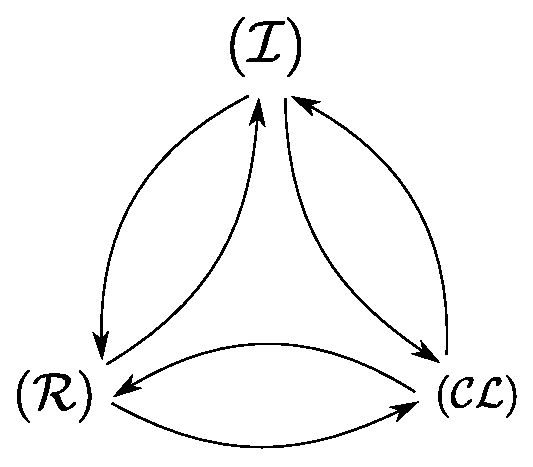
\includegraphics[scale=0.5]{Figures/Chapter1/equiv_def_2.eps}
    \caption{The equivalence of matroids defined by the independence $(\Ic)$,
    rank $(\Rc)$, and closure $(\Cc\Lc)$ axioms.}
    \label{fig_1.8}
\end{figure}

We can make one more definition for a matroid.

\begin{definition}
    Let $M$ be a matroid on a set  $E$. We define the  \textbf{nullity} of a set
    $X$ of  $M$ to be:
    \begin{equation*}
        \nul{X}=|X|-\rank{X}
    \end{equation*}
\end{definition}

One could define a matroid in terms of the nullity of its sets, however, doing
so shows that the axiom system for nullity is precisely that for rank
functiions. This makes the nullity of a matroid $M$ a rank function.
